\section{Methodology}
The initial phase of the internship involved familiarizing ourselves with the datasets we intended to explore.
Throughout the internship, we conducted two projects in parallel: one utilizing the Folktables dataset \cite{folktables} and the other utilizing the Titan dataset \cite{titandataset}. The first project focused on auditing fairness and bias in machine learning models by applying classical XAI methods to tabular data. The second project focused on weather prediction and the adaptation of these XAI methods for complex, high-dimensional data.

This parallel approach served a strategic purpose: to first explore the capability of methods like Anchors to explain individual predictions and reveal model bias on a simpler, more interpretable tabular dataset. The insights gained from this controlled environment were then leveraged to guide our efforts in tracking vulnerable areas and adapting XAI techniques for the multi-dimensional domain of meteorological data.



\subsection{Anchors Method}
\label{sec:anchors-formalization}
It's important to make clear how the method works and the precision and coverage measures for the followings sub-sections.

Following Ribeiro's formalization of the Anchors method \cite{anchors-ribeiro}, we consider a binary classifier $f : \mathcal{X} \rightarrow \{0, 1\}$. For a given instance $x$, the objective is to find a predicate $A$ that explains the prediction $f(x)$ by identifying a minimal set of decisive features.

A predicate $A$ is deemed a valid anchor if it meets a precision threshold, meaning it guarantees the model's output is consistent under local perturbation. Precision is formally defined as:
\begin{equation}
\text{prec}(A) = \mathbb{E}_{D(z|A)} [\mathbf{1}_{f(x) = f(z)}]
\label{eq:prec-anchors}
\end{equation}
where $D(\cdot|A)$ is the conditional distribution of inputs satisfying $A$. The anchor condition is satisfied with high confidence if $P(\text{prec}(A) \geq \tau) \geq 1 - \delta$.

It can be remarked that several sets of conditions can be considered as anchors. To select the most impactful and parsimonious explanation for end-users, the method introduces a coverage measure. The coverage of $A$ is defined as the probability that the predicate holds under the data distribution:
\begin{equation}
\text{cov}(A) = \mathbb{E}_{D(z)} [A(z)]
\label{eq:cov-anchors}
\end{equation}

For a given data distribution $D$, parameters $\tau$ and $\delta$, the optimal anchor is the one with maximum coverage subject to the precision constraint:
\begin{equation}
\arg \max_{A} {\text{cov}(A) \mid P(\text{prec}(A) \geq \tau) \geq 1 - \delta }
\label{eq:max-cov-anchors}
\end{equation}

%%%%%%%%%%%%%%%%%%%%%%%%%%%%%%%%%%%%%%%%%%%%%%%%%%%%%%%%%%%%%%%%%%%%%%%%%%%%%%%%%%%%%%%%%%%%%%%%%%%%%%%%%%%%%%%%%%%%%%%
%%%%%%%%%%%%%%%%%%%%%%%%%%%%%%%%%%%%%%%%%%%%%%% FOLKTABLES  %%%%%%%%%%%%%%%%%%%%%%%%%%%%%%%%%%%%%%%%%%%%%%%%%%%%%%%%%%%
%%%%%%%%%%%%%%%%%%%%%%%%%%%%%%%%%%%%%%%%%%%%%%%%%%%%%%%%%%%%%%%%%%%%%%%%%%%%%%%%%%%%%%%%%%%%%%%%%%%%%%%%%%%%%%%%%%%%%%%

\subsection{Tabular Data}
In this initial work done with Benoît and Jean-Michel we used the Folktables dataset \cite{folktables-ding} to apply the Anchors XAI method and try to identify new ways to detect unfairness related to sensitive variables.

The idea here was to explore Anchors, a method that is under-explored in comparison to SHAP. The Anchors method can be interesting for detecting the features taken into account in the decision-making process that maintain the result for a given individual in the dataset. As a perturbation-based method, it replicates the individual locally and verifies which features are responsible for maintaining the model's prediction.

In the case of the Folktables dataset, we wanted to investigate the \textit{SEX} feature as the sensitive variable, to see if the Anchors method could identify it as a decisive feature in the model's prediction.

\subsubsection{The Folktables Dataset}
The Folktables dataset, used in this part of the study, was derived from the 2018 Census of the United States of America (USA). For manipulating this dataset we used the Python library \cite{folktables}, which provides modules for data extraction tailored to specific prediction tasks. The prediction target we used was ACSIncome, meaning the machine learning model was designed to predict an individual's income bracket. The library defines True predictions for those who receive more than \$50,000 and False for those who receive less.

The variables of the dataset are described in Table \ref{tab:folktables-variables}, and their range of values can be consulted in the documentation \cite{folktables-ding}.

\begin{table}[h]
\centering
\caption{Folktables Dataset Features}
\label{tab:folktables-variables}
\begin{tabular}{lll}
\hline
\textbf{Feature code} & \textbf{Description} \\
\hline
AGEP & Age \\
COW & Class of Worker \\
SCHL & Educational Attainment \\
MAR & Marital Status \\
OCCP & Occupation \\
POBP & Place of Birth \\
RELP & Relationship \\
WKHP & Usual Hours Worked Per Week past 12 Months \\
SEX & Sex \\
RAC1P & Recoded detailed race code \\
\hline
\end{tabular}
\end{table}

\subsubsection{Training Data}
For our analysis, we used data covering the entire United States, as well as data from three of the most populous states: California, Texas, and New York. Each subset of data was trained using four widely adopted machine learning algorithms:

\begin{itemize}
	\item XGBoost (eXtreme Gradient Boosting) – A highly efficient and scalable implementation of gradient boosting, known for its performance in structured data tasks. We leveraged its ability to handle missing values and feature importance estimation.
	
	\item Logistic Regression – A classical linear model for binary and multiclass classification. Despite its simplicity, it served as a strong baseline, particularly for interpreting feature coefficients.
	
	\item Hist Gradient Boosting (Skrub's Scikit-learn implementation) – A fast and memory-efficient gradient-boosting variant that bins input features, making it suitable for large datasets while maintaining competitive accuracy.
	
	\item Simple Neural Network – A feedforward neural network with a limited number of layers to assess whether deeper architectures could capture nonlinear patterns beyond what tree-based models achieved.
\end{itemize}


The algorithms were used for classification tasks to predict whether income was higher (True) or lower (False) than \$50,000.

\subsubsection{Fairness Metrics}
After training the models, we evaluated their performance using accuracy and fairness metrics as explained below:

\begin{itemize}
	\item \textbf{Accuracy}: The proportion of correct predictions (both true positives and true negatives) among all predictions.

	\item \textbf{Disparate Impact (DI)}: Measures the ratio between the proportion of positive outcomes for the protected group (women) versus the privileged group (men). Values close to 1 indicate fairness, while values below 1 suggest bias against the protected group.

	\item \textbf{Equality of Odds}: Examines whether both groups have equal true positive rates and equal false positive rates. Values closer to 1 indicate better fairness.

	\item \textbf{Sufficiency}: Assesses whether the probability of the true outcome is the same across groups given the predicted outcome. Values closer to 1 indicate better fairness.
\end{itemize}

We can see on Table \ref{tab:folktables-results} the results comparing the four models in the three states.

Each model was trained on the training data of the state (indicated in the second column), and the fairness metrics were calculated by comparing them to the test data of the state or the full data of the USA (indicated in the third column) to provide both a local and global comparison.

\begin{table}[h]
\centering
\caption{Model Performance Comparison Across States (Accuracy and Fairness Metrics)}
\label{tab:folktables-results}
\resizebox{\textwidth}{!}
{
\begin{tabular}{llcccccc}
\toprule
\textbf{Model} & \textbf{Training} & \textbf{Testing} & \textbf{Accuracy} & \textbf{Disparate Impact} & \textbf{Equality of Odds} & \textbf{Sufficiency} \\
\midrule
\rowcolor{gray!10}
\multirow{6}{*}{Logistic Regression} 
& \multirow{2}{*}{CA} & CA & 0.56 & 0.67 & 0.84 & 0.95 \\
& & USA & 0.52 & 0.66 & 0.88 & 0.86 \\
\cmidrule(lr){2-7}
& \multirow{2}{*}{TX} & TX & 0.52 & 0.46 & 0.65 & 0.90 \\
& & USA & 0.51 & 0.46 & 0.67 & 0.95 \\
\cmidrule(lr){2-7}
& \multirow{2}{*}{NY} & NY & 0.51 & 0.66 & 0.82 & 0.93 \\
& & USA & 0.52 & 0.64 & 0.86 & 0.88 \\
\midrule

\rowcolor{gray!10}
\multirow{6}{*}{XGBoost} 
& \multirow{2}{*}{CA} & CA & 0.64 & 0.72 & 0.91 & 0.96 \\
& & USA & 0.58 & 0.67 & 0.92 & 0.90 \\
\cmidrule(lr){2-7}
& \multirow{2}{*}{TX} & TX & 0.60 & 0.58 & 0.83 & 0.93 \\
& & USA & 0.58 & 0.58 & 0.85 & 0.95 \\
\cmidrule(lr){2-7}
& \multirow{2}{*}{NY} & NY & 0.61 & 0.75 & 0.92 & 0.96 \\
& & USA & 0.57 & 0.67 & 0.92 & 0.90 \\
\midrule

\rowcolor{gray!10}
\multirow{6}{*}{HistGradientBoosting} 
& \multirow{2}{*}{CA} & CA & 0.63 & 0.71 & 0.90 & 0.94 \\
& & USA & 0.58 & 0.67 & 0.92 & 0.90 \\
\cmidrule(lr){2-7}
& \multirow{2}{*}{TX} & TX & 0.61 & 0.54 & 0.78 & 0.96 \\
& & USA & 0.58 & 0.56 & 0.83 & 0.97 \\
\cmidrule(lr){2-7}
& \multirow{2}{*}{NY} & NY & 0.60 & 0.68 & 0.89 & 0.97 \\
& & USA & 0.58 & 0.64 & 0.90 & 0.91 \\
\midrule

\rowcolor{gray!10}
\multirow{6}{*}{Neural Network} 
& \multirow{2}{*}{CA} & CA & 0.52 & 0.88 & 1.03 & 0.85 \\
& & USA & 0.46 & 0.65 & 0.86 & 0.86 \\
\cmidrule(lr){2-7}
& \multirow{2}{*}{TX} & TX & 0.50 & 0.61 & 0.87 & 0.94 \\
& & USA & 0.49 & 0.77 & 0.96 & 0.81 \\
\cmidrule(lr){2-7}
& \multirow{2}{*}{NY} & NY & 0.51 & 0.76 & 0.93 & 0.92 \\
& & USA & 0.48 & 0.66 & 0.88 & 0.87 \\
\bottomrule
\end{tabular}%
}
\end{table}

As the results with the most contrast are shown for the state of Texas, we will focus on these results for the discussion in the report, but the results for California and New York will be in the Appendix (Section \ref{ap:Opt}).

In Figures \ref{fig:roc_tx}, \ref{fig:roc_ca}, and \ref{fig:roc_ny}, we can see the ROC curves of the models applied to the Texas, California, and New York subsets of the data, respectively.

\begin{figure}[h]
    \centering
    \begin{subfigure}[b]{0.48\textwidth}
        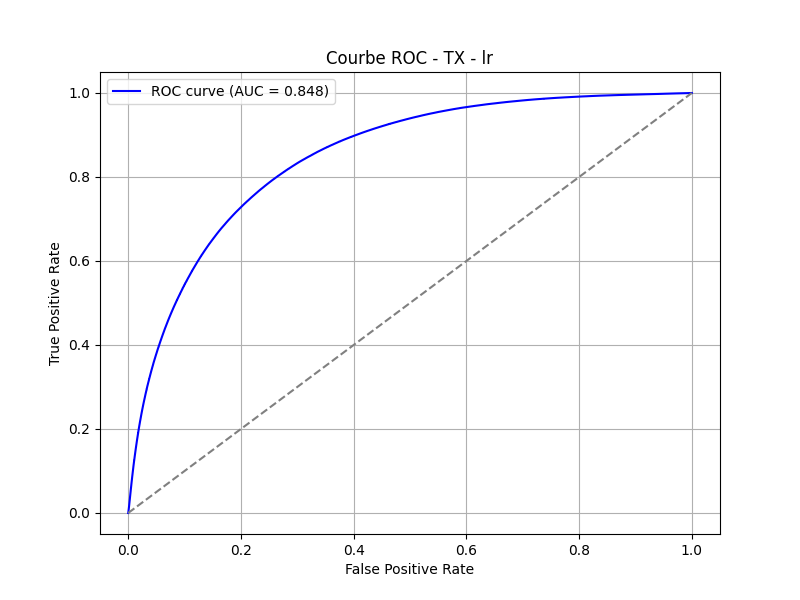
\includegraphics[width=\textwidth]{Images/curve_roc_folktables/roc_curve_TX_lr.png}
        \caption{Curve ROC (AUC = 0.848): model = Logistic Regression}
        \label{fig:TX_lr}
    \end{subfigure}
    \hfill
    \begin{subfigure}[b]{0.48\textwidth}
        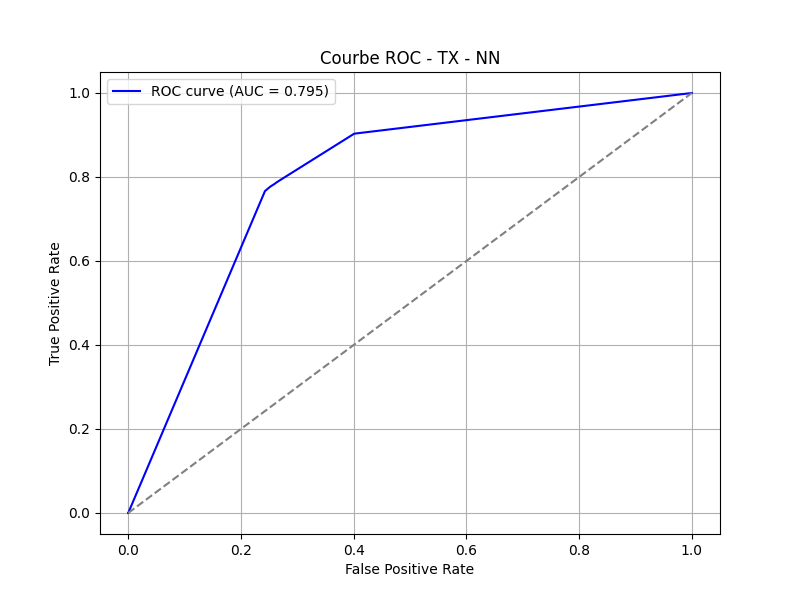
\includegraphics[width=\textwidth]{Images/curve_roc_folktables/roc_curve_TX_NN.png}
        \caption{Curve ROC (AUC = 0.795): model = Neural Network}
        \label{fig:TX_nn}
    \end{subfigure}

    \begin{subfigure}[b]{0.48\textwidth}
        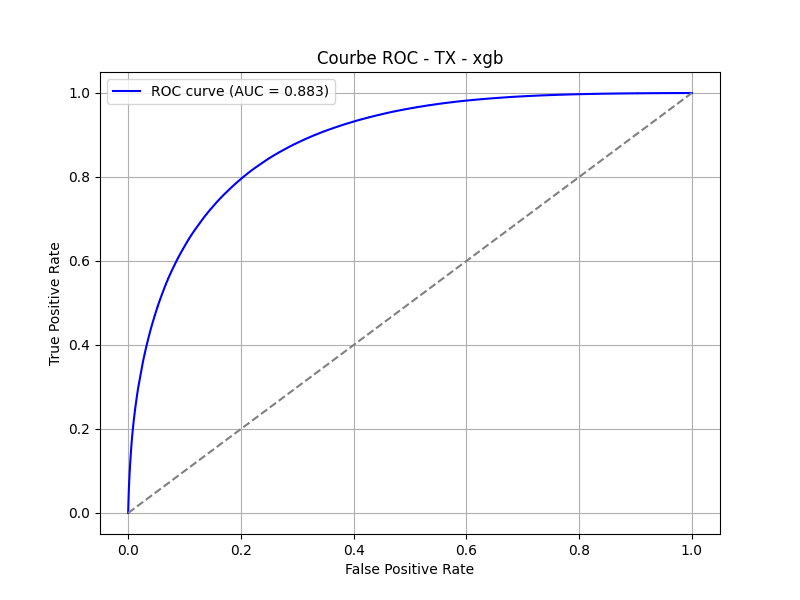
\includegraphics[width=\textwidth]{Images/curve_roc_folktables/roc_curve_TX_xgb.png}
        \caption{Curve ROC (AUC = 0.883): model = XGBoost}
        \label{fig:TX_xgb}
    \end{subfigure}
    \hfill
    \begin{subfigure}[b]{0.48\textwidth}
        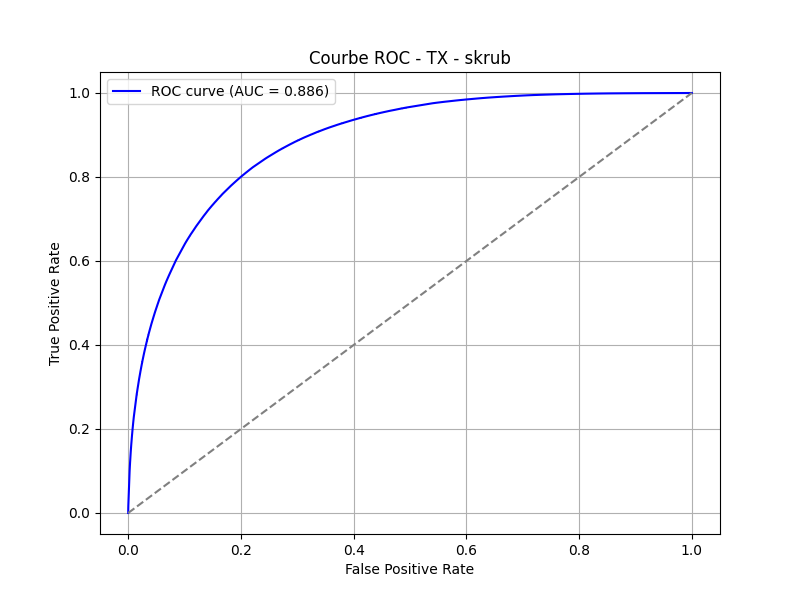
\includegraphics[width=\textwidth]{Images/curve_roc_folktables/roc_curve_TX_skrub.png}
        \caption{Curve ROC (AUC = 0.886): model = HistGradientBoosting}
        \label{fig:TX_skrub}
    \end{subfigure}
    \caption{Comparison of the models trained on the sub dataset of the Texas state}
    \label{fig:roc_tx}
\end{figure}

First, we can see the difference in performances between the models.
In the ROC curve graphics \ref{fig:roc_tx}, \ref{fig:roc_ca}, and \ref{fig:roc_ny}, we can see how XGBoost and HistGradientBoosting outperform the Neural Network, and how Logistic Regression remains average but still does not surpass the others.
Also note that the models with higher accuracy (fourth column) in Table \ref{tab:folktables-results} are XGBoost and HistGradientBoosting.

Second, we can now analyse the fairness metrics in columns five, six, and seven.
It is important to note that the fairness threshold for these metrics, as established by \cite{di-besse}, is 0.8. Values above 0.8 (and closer to 1) are generally considered to indicate fair predictions, while values below this threshold suggest varying degrees of unfairness.
Note that the Equality of Odds and Sufficiency metrics reach higher levels, all of them above 0.8. However, when looking at Disparate Impact (DI), we see a discrepancy from the reference values, with them staying on average 2 percentage points lower.
We interpret this low DI as indicating a discrepancy between women and men who receive more than \$50,000, showing a disadvantage for women in this case.

\subsubsection{Applying XAI Methods}
\label{met:fairness-xai}

After a short analysis of the DI metric for XGBoost and HistGradientBoosting, it is clear that there is a proven bias in the model's prediction. But knowing there is a bias is not enough, so we started using two XAI methods to try to find more information about the bias and try to identify a profile of the individuals who are being discriminated against by the model.

We employed the Anchors method \cite{anchors-ribeiro} to generate and export explanations, aiming to identify the features that were most decisive for the model's predictions.
For the sake of comparison, we also generated and exported the SHAP values of the subsets for further analysis.

We will refer to a \textbf{gendered anchor} when the generated Anchors explanation contains 'SEX' in its list of features, which is the sensitive variable we are analysing. In a similar way, we will refer to \textbf{gendered SHAP values} when the generated SHAP explanation contains 'SEX' at the top of the feature ranking.

\begin{figure}[h]
    \centering
    \begin{subfigure}[b]{0.9\textwidth}
        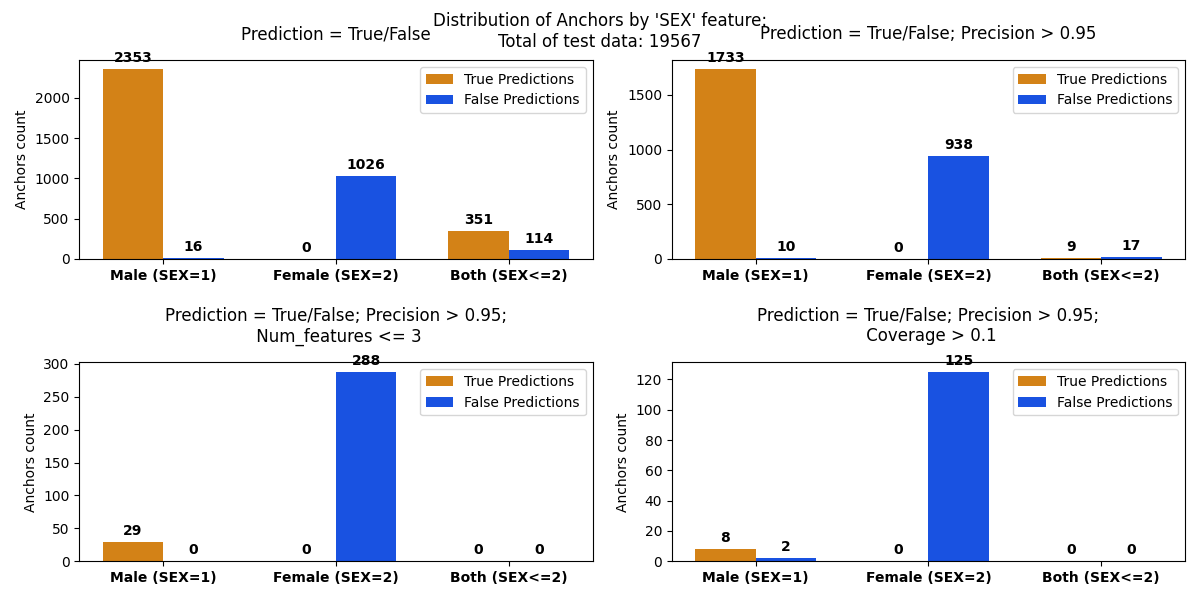
\includegraphics[width=\textwidth]{Images/distribution_folktables/pca_xg_ca_anchors.png}
        \caption{Model: XGBoost, XAI method: Anchors}
        \label{fig:distr_xg_ca_anchors}
    \end{subfigure}
    \hfill
    \begin{subfigure}[b]{0.9\textwidth}
        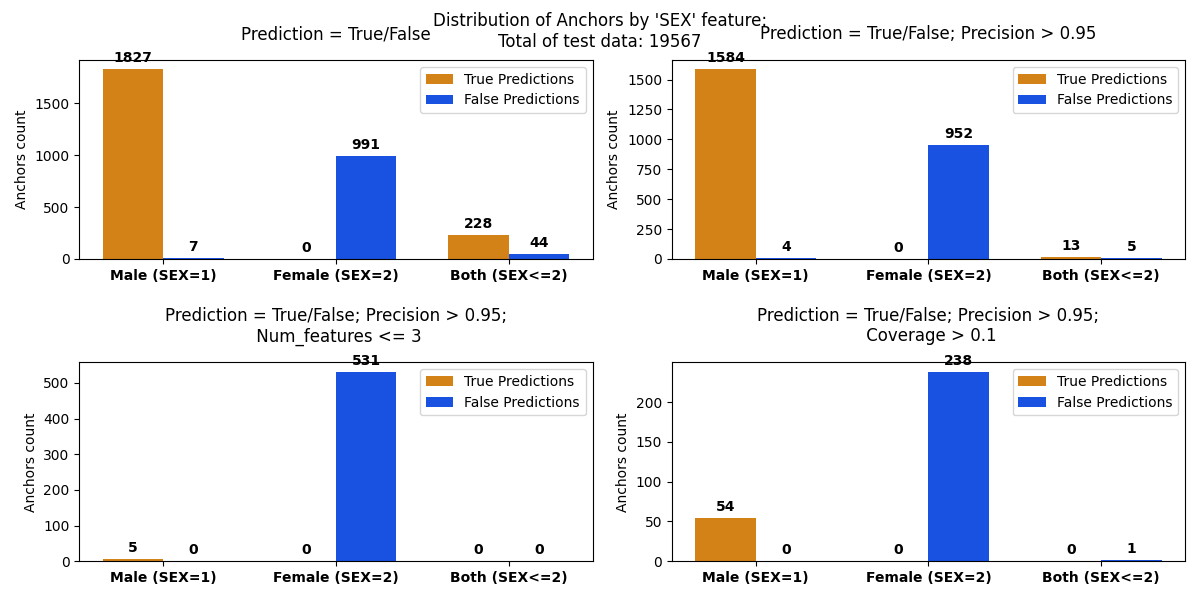
\includegraphics[width=\textwidth]{Images/distribution_folktables/pca_skrub_ca_anchors.png}
        \caption{Model: HistGradientBoosting, XAI method: Anchors}
        \label{fig:distr_skrub_ca_anchors}
    \end{subfigure}
    \caption{Comparison of the gendered explanations between True and False predictions in the California state (Part 1)}
 \end{figure}

\begin{figure}[h]
    \ContinuedFloat
    \begin{subfigure}[b]{0.9\textwidth}
        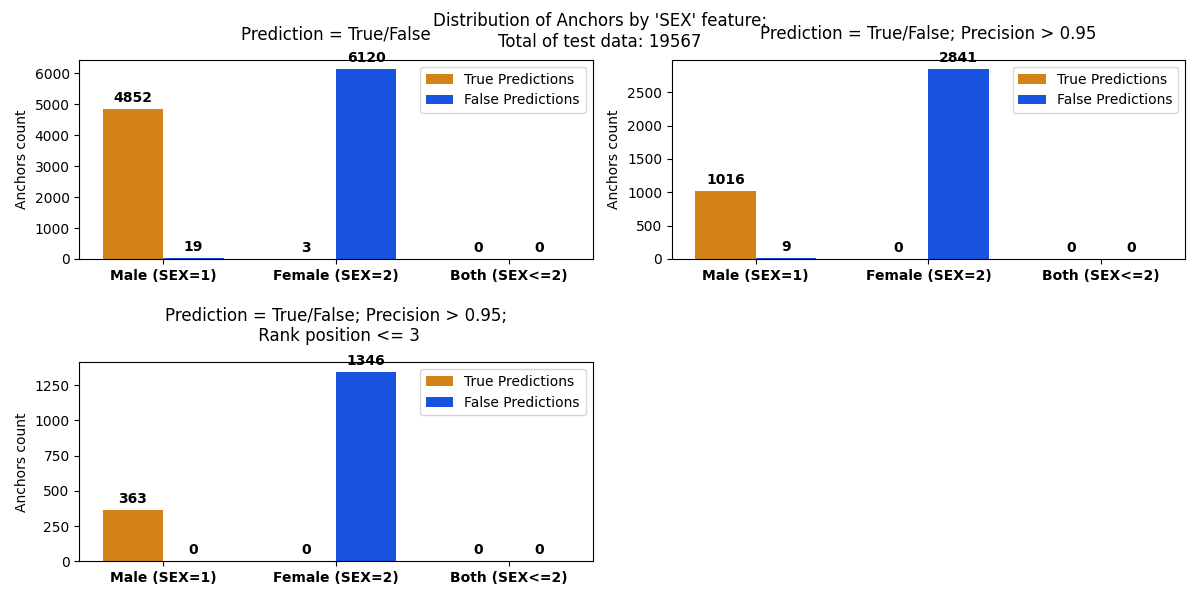
\includegraphics[width=\textwidth]{Images/distribution_folktables/pca_xg_ca_shap.png}
        \caption{Model: XGBoost, XAI method: SHAP}
        \label{fig:distr_xg_ca_shap}
    \end{subfigure}
    \hfill
    \begin{subfigure}[b]{0.9\textwidth}
        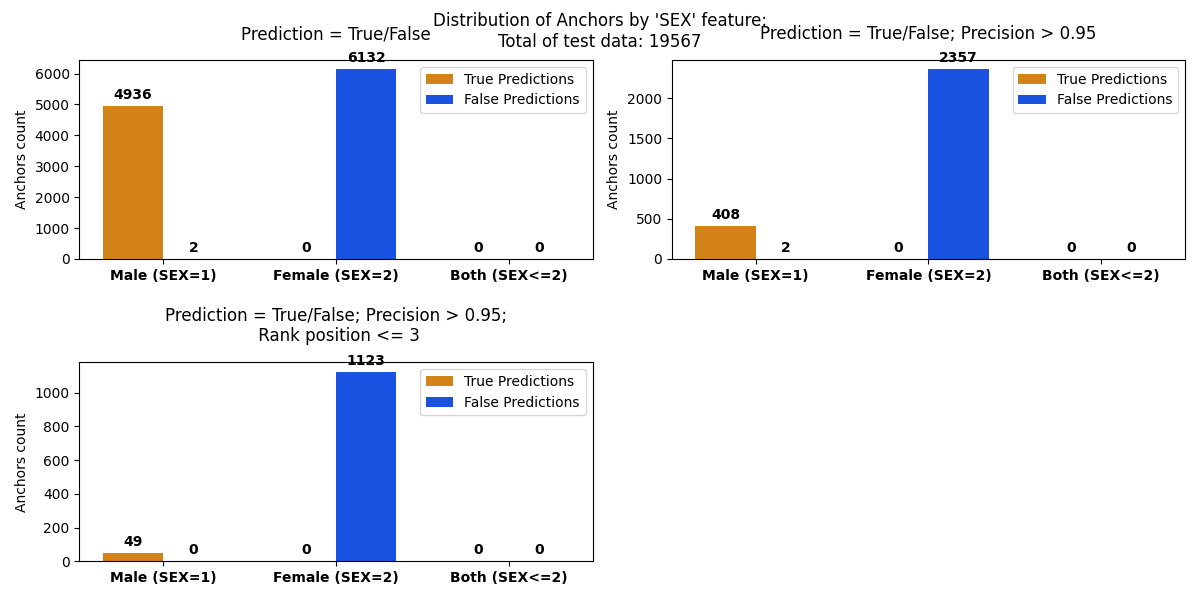
\includegraphics[width=\textwidth]{Images/distribution_folktables/pca_skrub_ca_shap.png}
        \caption{Model: HistGradientBoosting, XAI method: SHAP}
        \label{fig:distr_skrub_ca_shap}
    \end{subfigure}
    \caption{Comparison of the gendered explanations between True and False predictions in the California state (Part 2)}
    \label{fig:distr_ca}
\end{figure}

\begin{figure}[h]
    \centering
    \begin{subfigure}[b]{0.9\textwidth}
        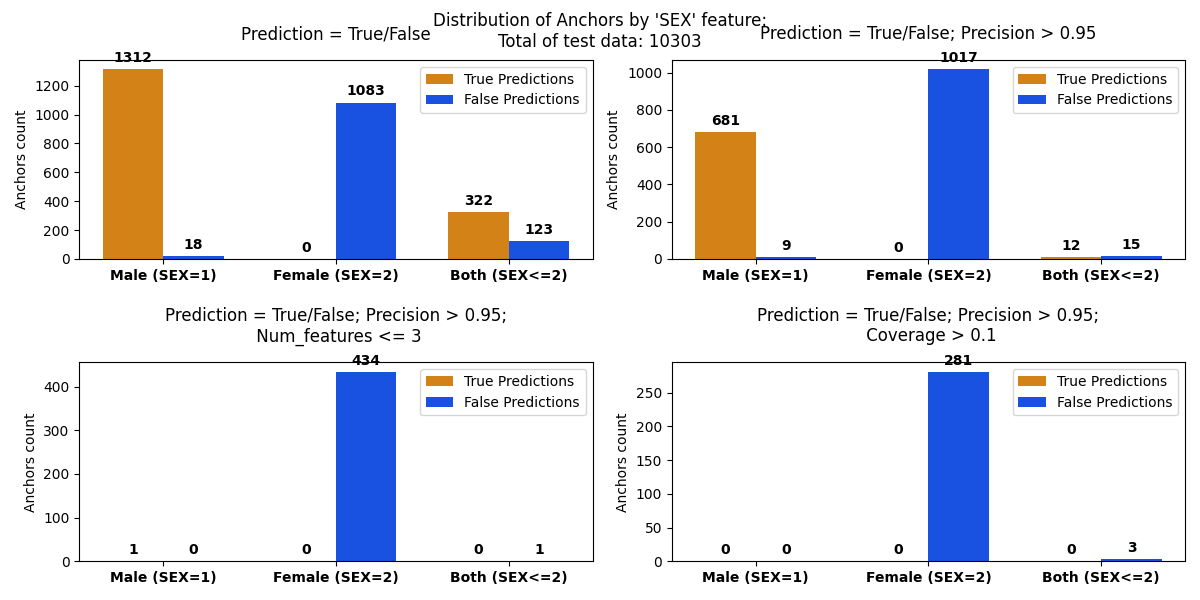
\includegraphics[width=\textwidth]{Images/distribution_folktables/pca_xg_ny_anchors.png}
        \caption{Model: XGBoost, XAI method: Anchors}
        \label{fig:distr_xg_ny_anchors}
    \end{subfigure}
    \hfill
    \begin{subfigure}[b]{0.9\textwidth}
        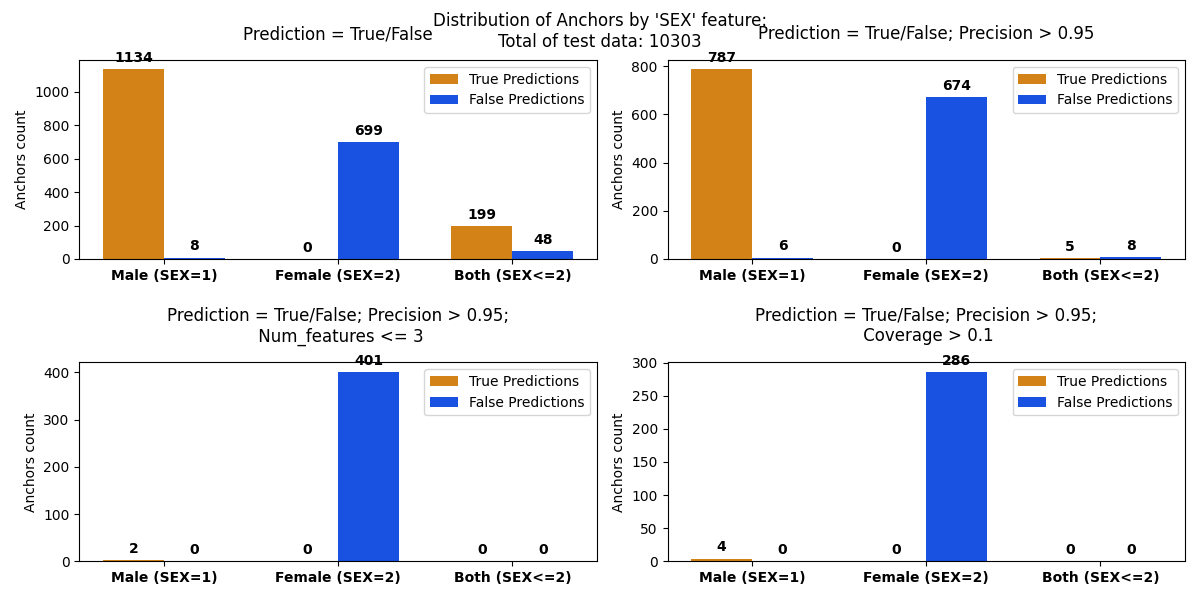
\includegraphics[width=\textwidth]{Images/distribution_folktables/pca_skrub_ny_anchors.png}
        \caption{Model: HistGradientBoosting, XAI method: Anchors}
        \label{fig:distr_skrub_ny_anchors}
    \end{subfigure}
    \caption{Comparison of the gendered explanations between True and False predictions in the New York state (Part 1)}
 \end{figure}

\begin{figure}[h]
    \ContinuedFloat
    \begin{subfigure}[b]{0.9\textwidth}
        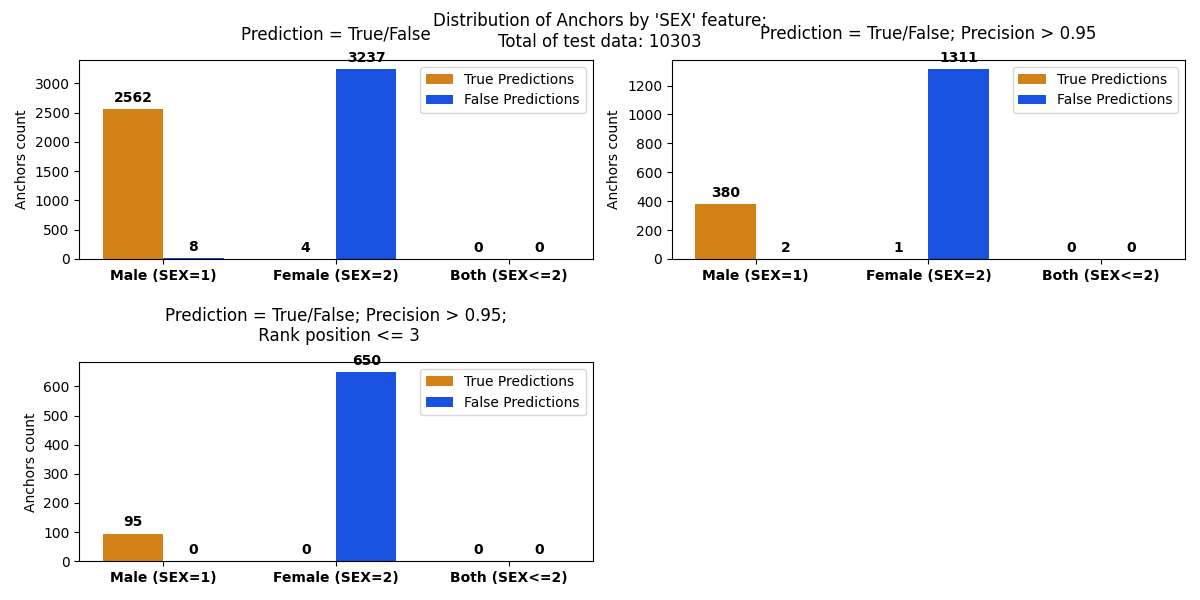
\includegraphics[width=\textwidth]{Images/distribution_folktables/pca_xg_ny_shap.png}
        \caption{Model: XGBoost, XAI method: SHAP}
        \label{fig:distr_xg_ny_shap}
    \end{subfigure}
    \hfill
    \begin{subfigure}[b]{0.9\textwidth}
        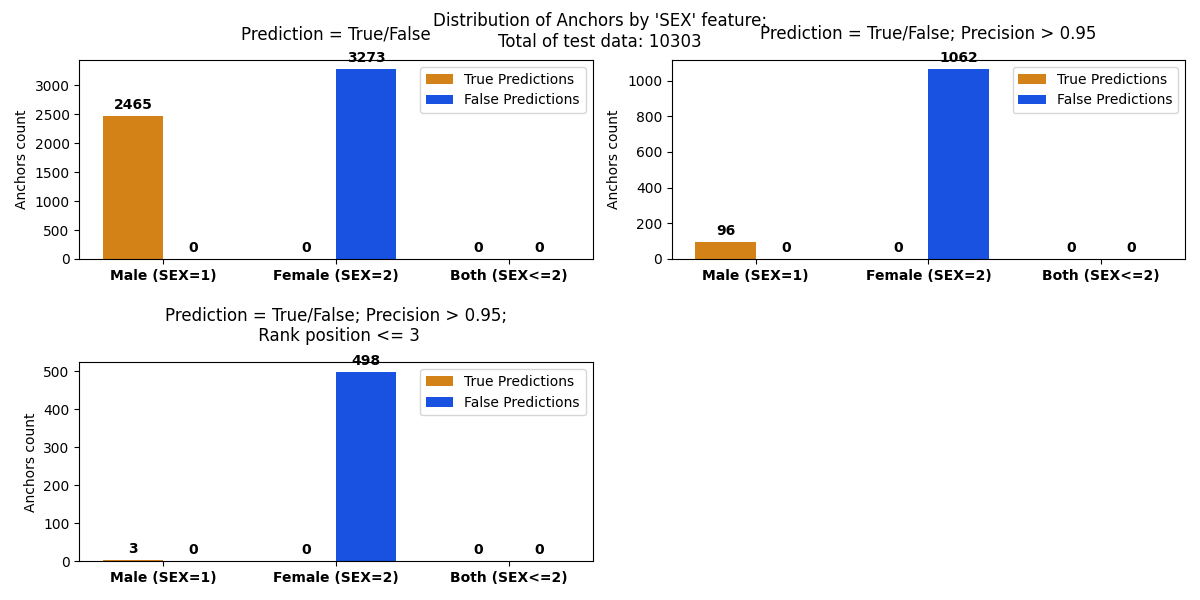
\includegraphics[width=\textwidth]{Images/distribution_folktables/pca_skrub_ny_shap.png}
        \caption{Model: HistGradientBoosting, XAI method: SHAP}
        \label{fig:distr_skrub_ny_shap}
    \end{subfigure}
    \caption{Comparison of the gendered explanations between True and False predictions in the New York state (Part 2)}
    \label{fig:distr_ny}
\end{figure}

Figures \ref{fig:distr_xg_tx_anchors} and \ref{fig:distr_skrub_tx_anchors} show the distribution of the 'SEX' variable in the Anchors generated for the test data of each state for the HistGradientBoosting and XGBoost models, respectively. In other words, the count of gendered anchors, broken down by the value of the 'SEX' variable (Male, Female, or instances where both values are included in the rule) and the model's prediction (True or False).
We also applied filters to understand better the impact of the anchor.

The plots are organized as follows:
\begin{enumerate}
	\item Distribution of True and False predictions among the gendered anchors.
	\item Distribution of True and False predictions (among the gendered anchors) with a precision higher than 95\%.
	\item Distribution of True and False predictions (among the gendered anchors) with a precision higher than 95\% and a rule size limited to three features, meaning a compact anchor.
	\item Distribution of True and False predictions (among the gendered anchors) with a precision higher than 95\% and coverage of the anchors higher than 10\% of the dataset.
\end{enumerate}

We tried to simulate the same tests with SHAP in Figures \ref{fig:distr_xg_tx_shap} and \ref{fig:distr_skrub_tx_shap}, showing the distribution of the 'SEX' variable among instances with positive SHAP values. We applied almost the same filters, apart from the coverage filter because SHAP values do not have a coverage attribute.
The plots are organized as follows:
\begin{enumerate}
	\item Distribution of True and False predictions among the instances with gendered (positive) SHAP values.
	\item Distribution of True and False predictions (among the instances with gendered SHAP values) with a precision higher than 95\%.
	\item Distribution of True and False predictions (among the instances with gendered SHAP values) with a precision higher than 95\% and in which the 'SEX' variable is in the top 3 of the SHAP value ranking.
\end{enumerate}

We can see the results for California and New York data in the Appendix, Figures \ref{fig:distr_ca} and \ref{fig:distr_ny}.

It was interesting to see how many explanations contained gendered anchors or SHAP values, meaning that the technique identified that feature as decisive for the prediction. This implies that if the value of 'SEX' changes, the prediction changes too.

We can also notice that the gendered explanations are divided mainly between women with a false model prediction and men with a true prediction. This reaffirms what the DI metric was showing: this imbalance in the proportion of True predictions for the protected group versus the privileged group.

Analyzing these plots, we discussed that it would be a good idea to analyse the profile of the test dataset to see how the Anchors and SHAP explanations are organized across different groups of people, and also to see which of these two strategies would be more interesting for our case study.

\FloatBarrier

%%%%%%%%%%%%%%%%%%%%%%%%%%%%%%%%%%%%%%%%%%%%%%%%%%%%%%%%%%%%%%%%%%%%%%%%%%%%%%%%%%%%%%%%%%%%%%%%%%%%%%%%%%%%%%%%%%%%%%%
%%%%%%%%%%%%%%%%%%%%%%%%%%%%%%%%%%%%%%%%%%%%%%%%   MÉTÉO   %%%%%%%%%%%%%%%%%%%%%%%%%%%%%%%%%%%%%%%%%%%%%%%%%%%%%%%%%%%%
%%%%%%%%%%%%%%%%%%%%%%%%%%%%%%%%%%%%%%%%%%%%%%%%%%%%%%%%%%%%%%%%%%%%%%%%%%%%%%%%%%%%%%%%%%%%%%%%%%%%%%%%%%%%%%%%%%%%%%%
\subsection{Multi-dimensional Data}
This part of the work was developed in collaboration with Laurent Risser and Météo France. Using the Titan dataset \cite{titandataset} provided by our partners, we explored the structure and composition of meteorological data. For this study, we focused on the Titan data collection for the year 2023.

Our first goal was to understand how meteorological data is organized and combined to produce forecasts. The initial phase involved studying the AROME and ARPÈGE data models and then training a model with a UNetR++-based neural network.

Establishing this solid foundation and successfully training the model was crucial for the next step: applying eXplainable AI (XAI) techniques to the predictions. The aim was to pinpoint the most important channels or specific areas in the input images that drive the model's predictions.

\subsubsection{The Titan Dataset}
This dataset is organized into hourly folders, each containing \textit{.npy} files for all 37 channels from the AROME \cite{arome} and ARPÈGE \cite{arpege} models (see Table \ref{tab:meteo_channels}). In essence, this structure provides a complete set of channel images for every hour (00h to 23h) of every day throughout the entire year of 2023.

Each of these channels represents a specific component of meteorological data, which can be categorized into AROME and ARPÈGE channels representing temperature, humidity, wind, and geopotential at different pressure levels.

\begin{table}[h]
\centering
\caption{Meteorological Data Channels and Their Properties}
\label{tab:meteo_channels}
\begin{tabular}{llll}
\hline
\textbf{Channel Number} & {Channel Name} & \textbf{Description} & \textbf{Altitude/Pressure Level} \\
\hline
1 & aro\_r2\_2m        & Arome relative humidity & 2 metre \\
2 & aro\_t2m\_2m       & Arome temperature & 2 metre \\
3 & aro\_t\_250hpa     & Arome temperature & 250 hPa \\
4 & aro\_t\_500hpa     & Arome temperature & 500 hPa \\
5 & aro\_t\_700hpa     & Arome temperature & 700 hPa \\
6 & aro\_t\_850hpa     & Arome temperature & 850 hPa \\
7 & aro\_tp\_0m        & Arome total precipitation & Surface \\
8 & aro\_u10\_10m      & Arome U wind component & 10 metre \\
9 & aro\_u\_250hpa     & Arome U wind component & 250 hPa \\
10 & aro\_u\_500hpa     & Arome U wind component & 500 hPa \\
11 & aro\_u\_700hpa     & Arome U wind component & 700 hPa \\
12 & aro\_u\_850hpa     & Arome U wind component & 850 hPa \\
13 & aro\_v10\_10m      & Arome V wind component & 10 metre \\
14 & aro\_v\_250hpa     & Arome V wind component & 250 hPa \\
15 & aro\_v\_500hpa     & Arome V wind component & 500 hPa \\
16 & aro\_v\_700hpa     & Arome V wind component & 700 hPa \\
17 & aro\_v\_850hpa     & Arome V wind component & 850 hPa \\
18 & aro\_z\_250hpa     & Arome geopotential & 250 hPa \\
19 & aro\_z\_500hpa     & Arome geopotential & 500 hPa \\
20 & aro\_z\_700hpa     & Arome geopotential & 700 hPa \\
21 & aro\_z\_850hpa     & Arome geopotential & 850 hPa \\
22 & arp\_t\_250hpa     & Arpege temperature & 250 hPa \\
23 & arp\_t\_500hpa     & Arpege temperature & 500 hPa \\
24 & arp\_t\_700hpa     & Arpege temperature & 700 hPa \\
25 & arp\_t\_850hpa     & Arpege temperature & 850 hPa \\
26 & arp\_u\_250hpa     & Arpege U wind component & 250 hPa \\
27 & arp\_u\_500hpa     & Arpege U wind component & 500 hPa \\
28 & arp\_u\_700hpa     & Arpege U wind component & 700 hPa \\
29 & arp\_u\_850hpa     & Arpege U wind component & 850 hPa \\
30 & arp\_v\_250hpa     & Arpege V wind component & 250 hPa \\
31 & arp\_v\_500hpa     & Arpege V wind component & 500 hPa \\
32 & arp\_v\_700hpa     & Arpege V wind component & 700 hPa \\
33 & arp\_v\_850hpa     & Arpege V wind component & 850 hPa \\
34 & arp\_z\_250hpa     & Arpege geopotential & 250 hPa \\
35 & arp\_z\_500hpa     & Arpege geopotential & 500 hPa \\
36 & arp\_z\_700hpa     & Arpege geopotential & 700 hPa \\
37 & arp\_z\_850hpa     & Arpege geopotential & 850 hPa \\
\hline
\end{tabular}
\end{table}

We conducted initial exploratory analyses in Python notebooks to understand the dataset. This involved loading the \textit{.npy} files representing the various channels, examining their structure, and interpreting the meteorological phenomena each one depicts. Examples of these channels are shown in Figure \ref{fig:titan-examples}.

\begin{figure}[h]
    \centering
    \begin{subfigure}[b]{0.3\textwidth}
        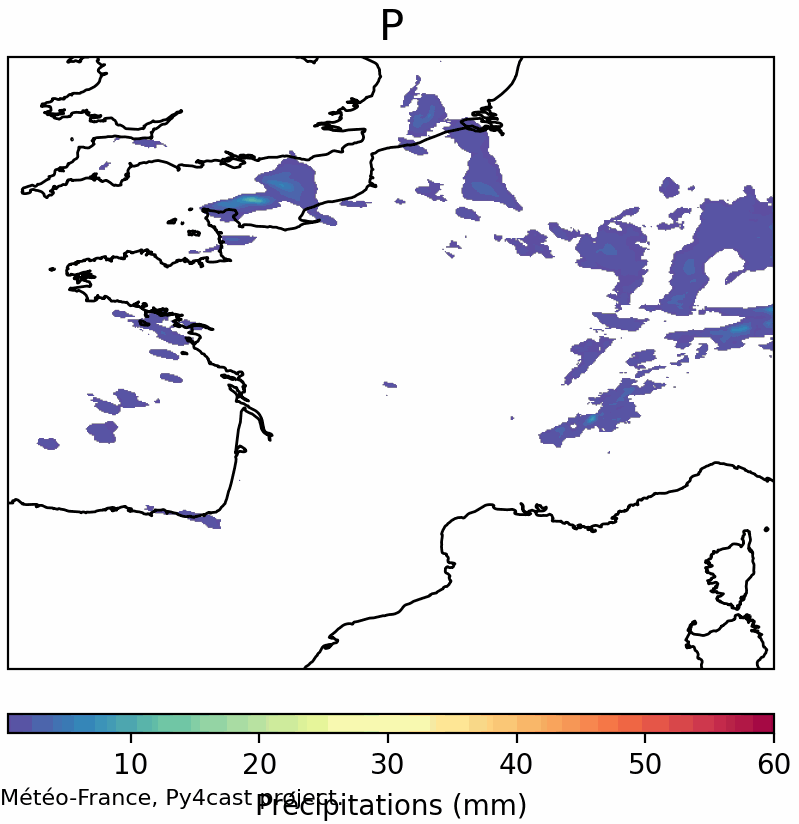
\includegraphics[width=\textwidth]{Images/titan_data_examples/2023111700_feature_aro_tp_0m.png}
        \caption{Feature aro\_tp\_0m}
        \label{fig:titan_aro_tp}
    \end{subfigure}
    \hfill
    \begin{subfigure}[b]{0.3\textwidth}
        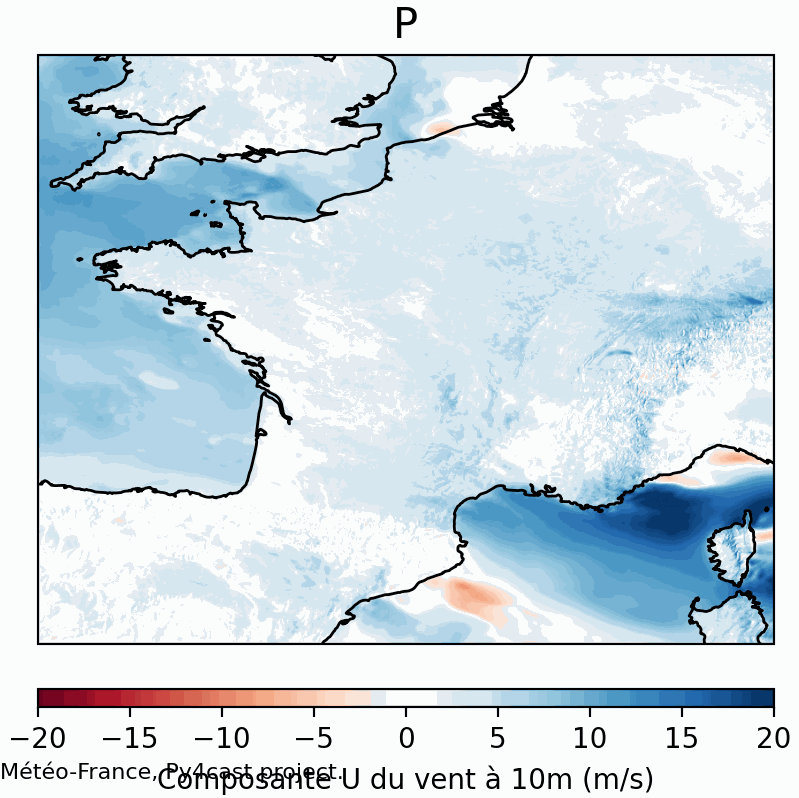
\includegraphics[width=\textwidth]{Images/titan_data_examples/2023111700_feature_aro_u10_10m.png}
        \caption{Feature aro\_u10\_10m}
        \label{fig:titan_aro_u10}
    \end{subfigure}
    \hfill
    \begin{subfigure}[b]{0.3\textwidth}
        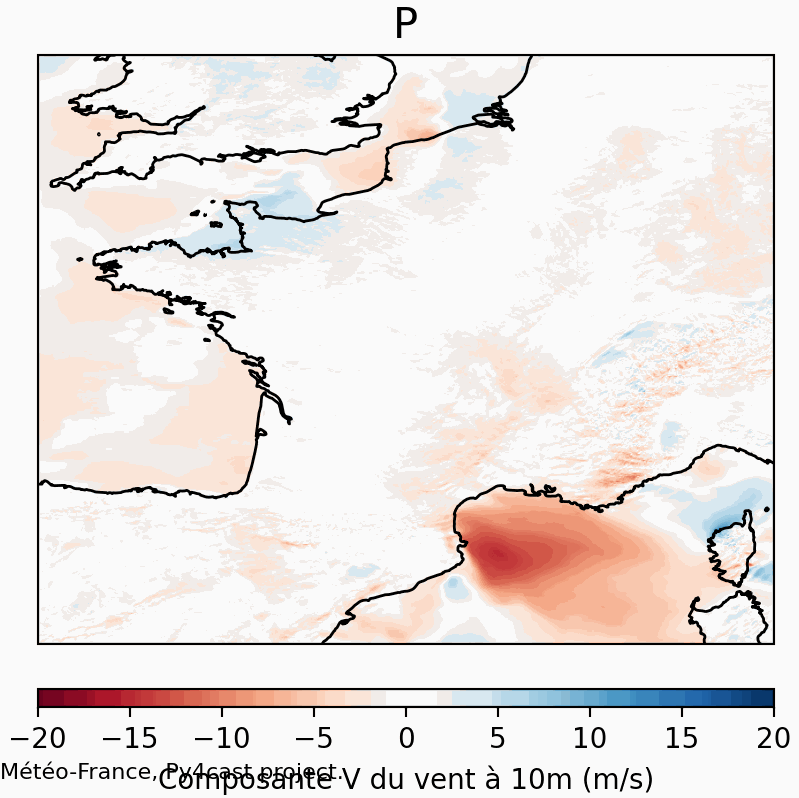
\includegraphics[width=\textwidth]{Images/titan_data_examples/2023111700_feature_aro_v10_10m.png}
        \caption{Feature aro\_v10\_10m}
        \label{fig:titan_aro_v10}
    \end{subfigure}
    \caption{Example of Titan image channels from 17/11/2023}
    \label{fig:titan-examples}
\end{figure}

By analyzing combinations of these components, one can identify and predict impending climatic events. The data can indicate future precipitation (rain or snow), temperature extremes (hot or cold), or the development of severe weather events like storms or flooding in the subsequent hours. For instance, in Figure \ref{fig:titan-examples}, we can identify regions with a high probability of rainfall and observe how wind patterns are likely to advect cloud cover to other areas.

\subsubsection{Training Data}
We first tried to use the \textit{py4cast} Python library \cite{py4cast} to run predictions, but these initial attempts were unsuccessful. As a result, we changed our strategy and began exploring the UNetR++ model using the MFAI Python library \cite{mfai}, developed by Météo France.

The MFAI library provides a framework for training advanced neural network models on meteorological data. We specifically employed it to implement a UNetR++ architecture \cite{unetrpp}. This model was chosen because it combines the strengths of a U-Net, known for its precise spatial segmentation in tasks like medical imaging, with a Vision Transformer (ViT). The ViT backbone is highly effective at capturing long-range dependencies and complex global patterns within the input data—a critical capability for understanding large-scale atmospheric dynamics. The "++" enhancements further refine the architecture for improved performance and efficiency, making it particularly well-suited for processing the high-dimensional, spatial-temporal data characteristic of meteorological fields.

This framework allowed us to investigate viable input and output configurations for weather prediction. It was instrumental in building an understanding of the complexity of meteorological data, the feasibility of training models on it, and the critical choices regarding parameters. The code for these initial experiments is available in the GitHub repository \cite{mfai-experiments}.

This exploratory phase led us to formulate key research questions to guide our work:
\begin{itemize}
\item \textbf{Prediction Target:} What specific meteorological phenomenon should we want to predict?
\item \textbf{Data Selection:} Which input channels are most relevant for this objective, and what should the model output?
\item \textbf{Data Integration:} How should we optimally combine the high-resolution AROME data with the global-scale ARPÈGE data?
\end{itemize}

Fundamentally, the input consists of an ensemble of channels relevant to a specific prediction task, which the model uses to predict the state of those channels at a future time step (e.g., the next hour).

Delving deeper into the integration of AROME and ARPÈGE data, we engaged with the key meteorological concept of training with boundary conditions. This technique is crucial because the AROME model provides high-resolution forecasts over a limited area (a fine mesh), while the ARPÈGE model offers coarser, global-scale (planetary) data. Operational weather forecasting often uses ARPÈGE data to define the boundary conditions for the higher-resolution AROME model. Formally, this can be conceptualized as follows:

Let $t$ be the present time and $t + 1$ be a future time.
\begin{itemize}
	\item Training without boundary conditions:
		\begin{itemize}
			\item Input: $aro_t$ (AROME at time $t$)
			\item Output: $aro_{t+1} - aro_t$ (The change in AROME from $t$ to $t+1$)
		\end{itemize}

	\item Training with boundary conditions:
		\begin{itemize}
			\item Input: $[aro_t, arp_t]$ (AROME and ARPÈGE at time $t$)
			\item Output: $aro_{t+1} - aro_t$ (The change in AROME from $t$ to $t+1$)
		\end{itemize}
\end{itemize}

Integrating the global ARPÈGE data ($arp_t$) as a boundary condition allows the model to incorporate large-scale atmospheric dynamics occurring outside the limited AROME domain, which is essential for generating more accurate predictions within the high-resolution area.

In summary, the data can be combined in two primary ways: a simpler approach using only AROME data, and a more precise, operational-style approach that leverages ARPÈGE data to provide essential boundary conditions.

To address the question of channel selection, we first needed to define a clear prediction objective. We chose precipitation (rain) prediction for its intuitive nature and direct impact. We know intuitively that rainfall is more likely in regions with high cloud cover or where wind patterns are converging and uplifting moisture.

\subsubsection{Using the \textit{py4cast} library}
The \textit{py4cast} library \cite{py4cast} is a Python framework developed by Météo France for short-term weather forecasting. It is specifically designed to work with high-resolution meteorological data from the AROME and ARPÈGE models. The library's core functionality involves processing images from these models to generate predictions for subsequent time steps, typically focused on a one-hour ahead forecast.

We worked in collaboration with Météo France using this library to train a neural network with the UNetR++ model \cite{unetrpp} and the Titan dataset \cite{titandataset} from 2023. This library is very recent, and it was highly valuable for both parties to have an external user test its capabilities. The main objective was to benefit from their library, as it already implemented the weather forecast training pipelines we required, complete with customizable input/output channels and built-in plotting functionalities.

However, as the documentation did not cover many aspects that an external user would not know initially, this process involved significant debugging and led to contributions aimed at improving the library's documentation and overall usability for external users. This challenge was a primary reason our research progress was slower than anticipated.

My role initially involved acting as a beta tester: reading the documentation and attempting to run the UNetR++ trainer. This was necessary because, in practice, Météo France's internal researchers were accustomed to using the library in a pre-configured environment. After several rounds of debugging in collaboration with their team, we successfully managed to run these models and generate the prediction images.


Being able to generate predictions allowed us to proceed with training the models. We trained two distinct models:
\begin{itemize}
	\item \textbf{Complete model}: A model trained with all the available image channels (listed in Table \ref{tab:meteo_channels}) as inputs.
	\item \textbf{Rain model}: A model trained with only the channels most relevant to precipitation (as explained above) as inputs, such as \textit{aro\_tp\_0m}, \textit{aro\_u10\_10m}, and \textit{aro\_v10\_10m}.
\end{itemize} 

\subsubsection{Applying XAI}
In order to apply XAI, we faced significant challenges. A primary obstacle was that standard XAI techniques like Anchors and SHAP are primarily designed for classification models, not regression tasks like weather prediction. Furthermore, applying these perturbation-based methods to multi-channel image data is non-trivial; perturbing individual pixels or channels could generate meteorologically nonsensical input images, rendering the explanations meaningless. We therefore needed to develop a technique that would address these issues.

Focusing on the Anchors framework, we will explore the properties explained in Section \ref{sec:anchors-formalization} to build a new proposition.

We elaborated two extensions of the Anchors formalization, which will be particularly useful for the weather forecasting problem.

\begin{itemize}
	\item Deterministic Precision Constraint: In scenarios where the amount of available data is sufficient to robustly represent the potential distribution $D(z|A)$, or when the estimation of $f(z)$ is computationally expensive, the following simplified optimization problem can be reasonably used:

	\begin{equation}
		\arg \max_{A} {\text{cov}(A) \mid \text{prec}(A) \geq \tau }
		\label{eq:extended-max-cov-anchors}
	\end{equation}

	\item Extension to Regression and Probabilistic Output: The original definition of precision (Eq. \ref{eq:prec-anchors}) is specific to classification tasks. For regression, or to assess the stability of prediction probabilities in classification, the precision measure can be extended as follows:
	
	\begin{equation}
		\text{prec}(A) = \mathbb{E}_{D(z|A)} [\mathbf{1}_{|f(x) - f(z)| > \tau}]
		\label{eq:extended-prec-anchors}
	\end{equation}

	where $\tau$ is a threshold above which the conditions of A are supposed to have a significant impact.
\end{itemize}

It is now crucial to define the specific subject of our explanations. Explaining the entire prediction $\widetilde{x_{t+1}}$ appears both technically intractable and, in our view, not particularly useful. Instead, we will focus on answering a more targeted question: why is $\widetilde{x_{t+1}}(i, j, c) \in R$? Here, $R$ represents a specific range of values. For instance, $(i, j)$ could denote the geographical coordinates of a city and $c$ the output channel representing the predicted rainfall in millimeters at that location for the next hour.

In this framework, defining $R = [ 1, +\infty [$ would allow us to explain why at least light rain is predicted locally. Alternatively, setting $R = [10, +\infty [$ would help explain the prediction of heavy rainfall.

To align with the classification framework established in Section \ref{sec:anchors-formalization}, we define a function $g_{i,j,c,R}(.)$ that transforms the regression output into a binary classification problem:
\begin{equation}
	g_{i,j,c,R}(\widetilde{x_{t+1}}) = \mathbf{1}_{\widetilde{x_{t+1}}(i, j, c) \in R}
\end{equation}

In summary, using Eq. \ref{eq:extended-max-cov-anchors}, we will explain the decisions $g_{i,j,c,R}(f(x_t))$ by evaluating the model on perturbed inputs $z$ similar to $x_t$. This approach raises two key questions:
\begin{itemize}
	\item Which channels of $z$ will be perturbed to generate the counterfactuals?
	\item Which types of conditions of $A$ can be considered on weather forecasting data, to formally measure the precisions and coverages of potentials anchors A?
\end{itemize}

Our two main difficulties in addressing the key questions above are:
\begin{itemize}
\item The dimensionality of the input $x_t$ is very large (with $p$ typically on the order of $500 \times 500 \times 20$).
\item Each model inference $f(z)$ or $f(x_t)$ requires a non-negligible amount of computational time.
\end{itemize}

Therefore, to generate pertinent explanations with reasonable computational resources, it is mandatory to sample perturbations $z$ using strong priors that guide the exploration towards meaningful differences from $x_t$.

What strategies can we use?
\begin{enumerate}
\item Leverage Spatial Structure: Unlike tabular data, we can exploit the spatial relationships between variables when defining predicates in $A$.
\item Define Clear Counterfactuals: The instances $z$ should be counterfactual versions of $x_t$, where the differences are explicitly defined by quantifiable relationships (e.g., concerning spatial locations, channel values, or local perturbations). The conditions in anchor $A$ must be able to formally express these relationships.
\item Focus on Local Neighborhood: Since the explanation targets a specific spatial location $(i, j)$, it is reasonable to sample $z$ by introducing differences within the neighborhood of $(i, j)$.
\item Utilize Domain Knowledge for Sampling: For each channel $c$—and potentially for each location $(i, j)$, hour, or season—domain knowledge can provide plausible value ranges for sampling $z$. Working with centered and reduced data (as is the case in py4cast) may simplify this generation process, as the range of potential values is broadly controlled and normalized.
\item Decouple Computation via a Table: The differences between each sampled $z$ and $x_t$ should be cataloged in a table. This approach would allow an external script to compute the Precision and Coverage measures for potential anchors $A$ using pre-computed model outputs. If executed properly, this method would require no modifications to the core py4cast code.
\end{enumerate}

\subsubsection{Proposed Solution}
We suppose that $g_{i,j,c,R}(f(x_t)) == 1$ and we want to explain why using anchors. We will sample $K$ different counterfactual observations ${z_k}$, for $k \in {1, \ldots , K}$, by generating perturbations based on the following quantified conditions:

\begin{itemize}
	\item \textbf{Center of Perturbation $(\widehat{i_k}, \widehat{j_k})$:} The epicenter of the perturbation should be close to the target location $(i, j)$ and lie within the spatial domain of the image. We can sample this center from a distribution, for instance $\widehat{i_k} \sim \mathcal{N}(i, \sigma_d)$ and $\widehat{j_k} \sim \mathcal{N}(j, \sigma_d)$, where $\sigma_d$ is a hyperparameter controlling the typical spatial scale of the perturbations. If the sampled coordinate falls outside the valid domain, it is projected to the nearest pixel on the grid.
	
	\item \textbf{Channel of Perturbation $\widehat{c_k}$:} The channel to be perturbed can be sampled uniformly from the available channels.
	
	\item \textbf{Perturbation Value $\widehat{v_k}$:} This defines the new value for the pixel at the chosen location and channel, i.e., $z_k(\widehat{i_k}, \widehat{j_k}, \widehat{c_k}) = \widehat{v_k}$. Assuming the channels of $x_t$ are centered and reduced, we can sample the new value from a distribution such as $\widehat{v_k} \sim \mathcal{N}(\mu, \sigma_v)$, where $\mu$ and $\sigma_v$ are hyperparameters. The maximum and minimum possible values for $\widehat{v_k}$ must be bounded by the physical limits (min/max) of the channel $\widehat{c_k}$ to ensure the generated counterfactual $z_k$ remains meteorologically plausible.
\end{itemize}

It can be remarked that altering the value of a single pixel in $x_t$ may have a negligible impact on the prediction $g_{i,j,c,R}(f(x_t))$ and often lacks physical realism. To address this, we introduce a second hyperparameter, $\sigma_e$, which models the spatial extent of the perturbation. The procedure for generating a counterfactual instance $z_k$ is then as follows:
\begin{itemize}
	\item \textbf{Unaffected Channels:} For all channels $c \neq \widehat{c_k}$, the data remains unchanged: $z_k(:, :, c) = x_t(:, :, c)$.
	
	\item \textbf{Mask Creation:} A mask $m \in \mathbb{R}^{I \times J}$ is generated. Its values are initially drawn from a 2D Gaussian distribution centered at $(\widehat{i_k}, \widehat{j_k})$ with covariance matrix $\begin{bmatrix} \sigma_e & 0 \ 0 & \sigma_e \end{bmatrix}$. These values are then linearly rescaled to the interval $[0, 1]$.
	
	\item \textbf{Application:} The perturbed channel $\widehat{c_k}$ in $z_k$ is created by a mask-based blending between the original values and the new value $\widehat{v_k}$:
	\begin{equation}
		z_k(\overline{i} , \overline{j} , \widehat{c_k}) = m(\overline{i} , \overline{j} ) * \widehat{v_k} + (1 - m(\overline{i} , \overline{j})) * x_t(\overline{i} , \overline{j}, \widehat{c_k})
		\label{eq:anchor-perturbation}
	\end{equation}
	for all $\overline{i} \in {1, \ldots, I}$ and $\overline{j} \in {1, \ldots, J}$.
\end{itemize}

Once all counterfactual observations ${z_k}$ are generated, we compute the corresponding model outputs $g_{i,j,c,R}(f(z_k))$. The anchor explanation process can then be performed by treating the set of perturbation parameters ($\widehat{i_k}, \widehat{j_k}, \widehat{c_k}, \widehat{v_k}$) and their outcomes $g_{i,j,c,R}(f(z_k))$ as tabular data for analysis.

% Falar sobre gradients e como nao conseguimos extrai-los por causa do Lightning